\documentclass[
11pt,%
tightenlines,%
twoside,%
onecolumn,%
nofloats,%
nobibnotes,%
nofootinbib,%
superscriptaddress,%
noshowpacs,%
centertags]%
{revtex4}
\usepackage{ljm}
\usepackage{listings}
\usepackage[utf8]{inputenc}
\usepackage[russian]{babel}

\lstset{
language=C++,
basewidth=0.5em,
xleftmargin=45pt,
xrightmargin=45pt,
basicstyle=\small\ttfamily,
keywordstyle=\bfseries\underbar,
numbers=left,
numberstyle=\tiny,
stepnumber=1,
numbersep=10pt,
showspaces=false,
showstringspaces=false,
showtabs=false,
frame=trBL,
tabsize=2,
captionpos=t,
breaklines=true,
breakatwhitespace=false,
escapeinside={\%*}{*)}
}

\begin{document}

\titlerunning{Meshes self-intersections elimination}
\authorrunning{Freylekhman et al.}

\title{Self-intersections elimination for unstructured surface computational meshes}

\author{\firstname{S.~A.}~\surname{Freylekhman}}
\email[E-mail: ]{freysa@jscc.ru}
\affiliation{Joint Supercomputer Center of the Russian Academy of Sciences -- branch of Scientific Research Institute of System Analysis of the Russian Academy of Sciences, Leninsky prospect 32a, Moscow, 119334, Russia}

\author{\firstname{A.~A.}~\surname{Rybakov}}
\email[E-mail: ]{rybakov@jscc.ru}
\affiliation{Joint Supercomputer Center of the Russian Academy of Sciences -- branch of Scientific Research Institute of System Analysis of the Russian Academy of Sciences, Leninsky prospect 32a, Moscow, 119334, Russia}

\firstcollaboration{(Submitted by TODO)} % Add if you know submitter.
%\lastcollaboration{ }

\received{TODO}

\begin{abstract}
Во время численного решения задачи обледенения трехмерного тела возникает проблема представления поверхности этого тела в процессе образования ледяного нароста.
Поверхность обтекаемого тела описывается неструктурированной поверхностной расчетной сеткой, ячейки которой являются треугольниками.
В процессе расчета обледенения ледяной нарост может принимать произвольные формы, а поверхностная сетка должна перестраиваться в соответствие с этим.
При этом в реальности нередки ситуации, когда отдельные части ледяного нароста могут соединяться друг другом, наслаиваться друг на друга, образуя пустоты и полости внутри ледяной массы.
В численном решении данная ситуация выражается в появлении самопересечений поверхностной сетки.
Возникновение самопересечений расчетной сетки делает невозможным продолжение вычислений на поверхности тела, поэтому самопересечения должны быть обнаружены и устранены.
Данная работа посвящена практическому алгоритму нахождения и устранения самопересечений неструктурированной поверхностной расчетной сетки при решении задачи обледенения обтекаемого тела.
\end{abstract}

\subclass{TODO} % Enter 2010 Mathematics Subject Classification.

\keywords{обледенение обтекаемого тела, неструктурированная поверхностная расчетная сетка, перестроение поверхности, самопересечение расчетной сетки}

\maketitle

\section{Introduction}

Расчет обледенения поверхности обтекаемого тела является важной практической задачей, необходимой для обеспечения функциональности и безопасности летательных аппаратов \cite{Myers, Farzaneh, Dong, Beaugendre}.
Компьютерное моделирование процессов обледенения может быть выполнено с использованием широкого набора инструментов, среди которых можно отметить FENSAP-ICE \cite{Bourgault}, LEWICE \cite{Wright}, OpenFOAM \cite{Beld}, AIPAC \cite{Domingos}, IceVision \cite{Aksenov} и другие.
Результатом проведения расчетов обледенения поверхности тела становятся значения массы (или объема льда), накопленного в той или иной ячейке расчетной сетки.
В соответствие с этой информацией поверхность тела должна быть перестроена таким образом, чтобы новая поверхность отражала характер и количественные показатели ледяного нароста.
Перестроение поверхности по значениям массы льда в ячейках расчетной сетки обычно выполняется итерационно (ледяной нарост моделируется последовательно с помощью отдельных слоев \cite{BourgaultCote, Fortin}).
Для обработки сложных участков поверхностей, впадин и изломов используются специальные методы сглаживания поверхности и перераспределения массы льда \cite{Thompson, Tong}.

Несмотря на все усилия, применяемые при перестроении поверхности, реальные расчетные сетки, которые используются в практических задачах, в процессе перестроения могут пересекать друг друга.
Это соответствует ситуациям, когда разные участки ледяного нароста при увеличении сталкиваются друг с другом, образуя внутренние полости.
Пересечение расчетных сеток порождает петли, которые оказываются скрытыми под внешней поверхностью, и наличие таких петель делает невозможным корректное продолжение расчетов.
Различные подходы у устранению самопересечений расчетных сеток можно найти в \cite{Charton, Jung, Skorkovska}.
Основной проблемой, с которой столкнулись авторы данной статьи при численном решении практических задач, стала сильно изломанная форма поверхности образующегося ледяного покрова и зачастую сильно вытянутые ячейки расчетной сетки ($\frac{max(a, b, c)}{min(a, b, c)} \gg 1$ для треугольных ячеек со сторонами $a$, $b$, $c$).
В данной статье была сделана попытка привести максимально упрощенный алгоритм устранения самопересечений для таких "плохих" расчетных сеток.

\section{Общая схема алгоритма устранения самопересечений расчетной сетки}

Перед определением общей схемы алгоритмы приведем описание неструктурированной поверхностной расчетной сетки.
Объектами такой сетки являются вершины (с ними ассоциированы три декартовы координаты $x$, $y$, $z$), ребра и треугольные ячейки.
При этом выполняются обязательные соглашения: каждое ребро соединяет ровно две вершины, каждая треугольная ячейка инцидентна трем вершинам и трем ребрам, ребро может быть инцидентно не более чем двум ячейкам.
Последнее требование позволяет разделить внутреннюю и внешнюю область поверхностьи, образованную парой ячеек, которые сходятся в некотором ребре.

\begin{figure}[h]
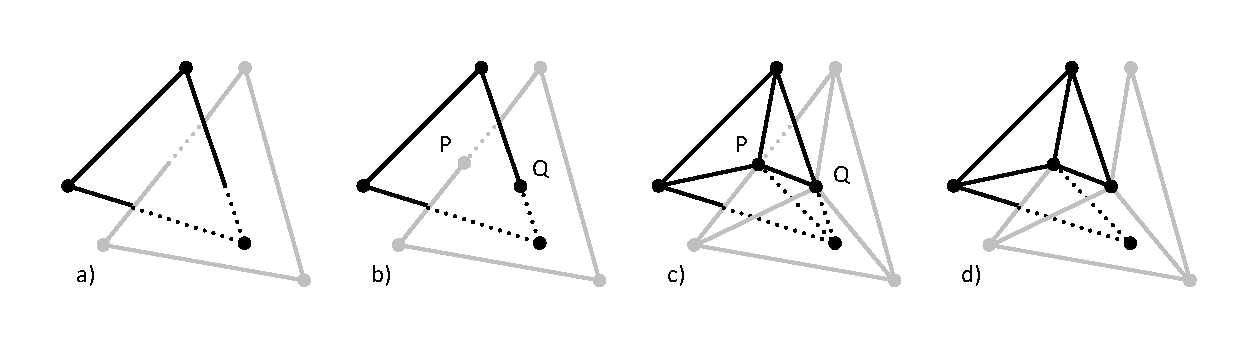
\includegraphics[width=1.0\textwidth]{pics/pic_algorithm_phases_s.pdf}
\captionstyle{center}\caption{Стадии устранения самопересечений.}\label{fig:pic_algorithm_phases_s}
\end{figure}

На рис.~\ref{fig:pic_algorithm_phases_s} представлены 4 фазы алгоритма устранения пересечений.
На первой фазе (рис.~\ref{fig:pic_algorithm_phases_s}, a) выполняется поиск всех пар ячеек (треугольников) которые пересекаются.
На второй фазе (рис.~\ref{fig:pic_algorithm_phases_s}, b) ищутся все точки пересечения треугольников (на данном рисунке показаны точки пересечения $P$ и $Q$).
На третьей фазе (рис.~\ref{fig:pic_algorithm_phases_s}, с) выполнятся разбиение пересекающихся треугольников на более мелкие таким образом, чтобы в получившейся измельченной сетке были только смежные по ребрам и вершинам треугольники (не было пересечений по внутренним точкам).
Очевидно, что после выполнения третьей фазы алгоритма в сетке могут образоваться ребра, инцидентные более чем двух ячейкам (на рис.~\ref{fig:pic_algorithm_phases_s}, с ребро $PQ$ инцидентно сразу четырем ячейкам).
Поэтому на четвертой фазе алгоритма (рис.~\ref{fig:pic_algorithm_phases_s}, d) осуществляется удаление лишних ячеек сетки (удаляются множества ячеек, которые образуют внутренние полости сетки).

Далее рассмотрим подробнее каждую из приведенных фаз алгоритма по-отдельности.

\section{Поиск пар потенциально пересекающихся треугольников}

\begin{figure}[h]
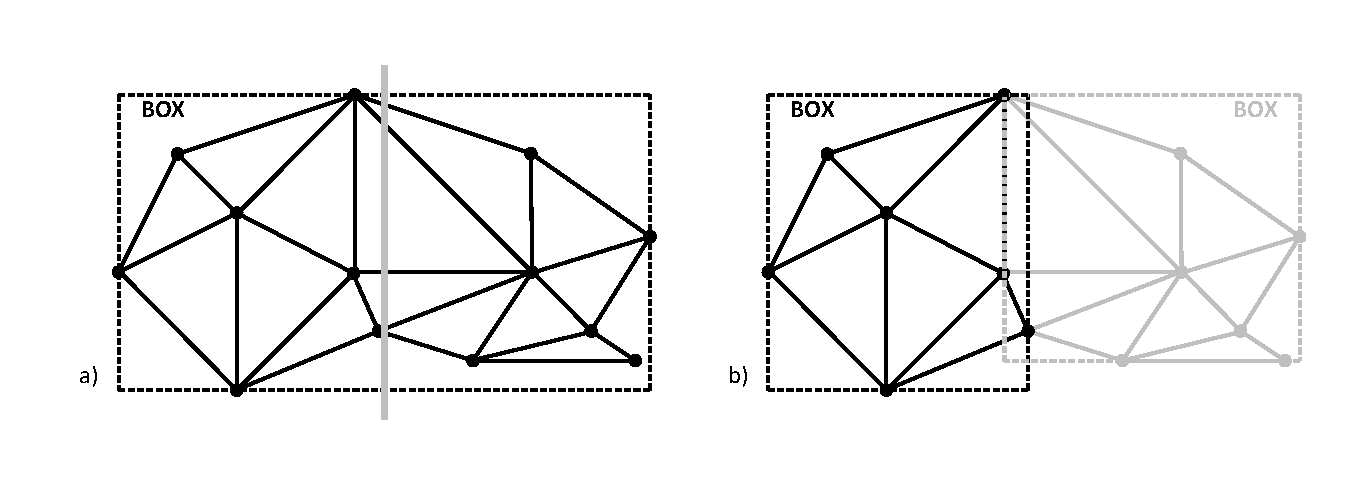
\includegraphics[width=1.0\textwidth]{pics/pic_triangles_cloud_s.pdf}
\captionstyle{center}\caption{Формирование облака треугольников.}\label{fig:pic_triangles_cloud_s}
\end{figure}

\section{Поиск точек пересечения треугольников}

\begin{figure}[h]
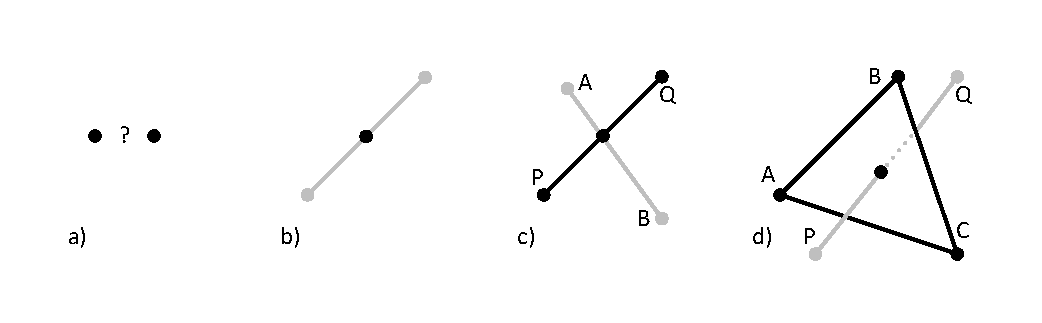
\includegraphics[width=1.0\textwidth]{pics/pic_intersection_s.pdf}
\captionstyle{center}\caption{Поиск точек пересечения разных геометрических примитивов.}\label{fig:pic_intersection_s}
\end{figure}

\section{Разбиение треугольников на более мелкие}

\begin{figure}[h]
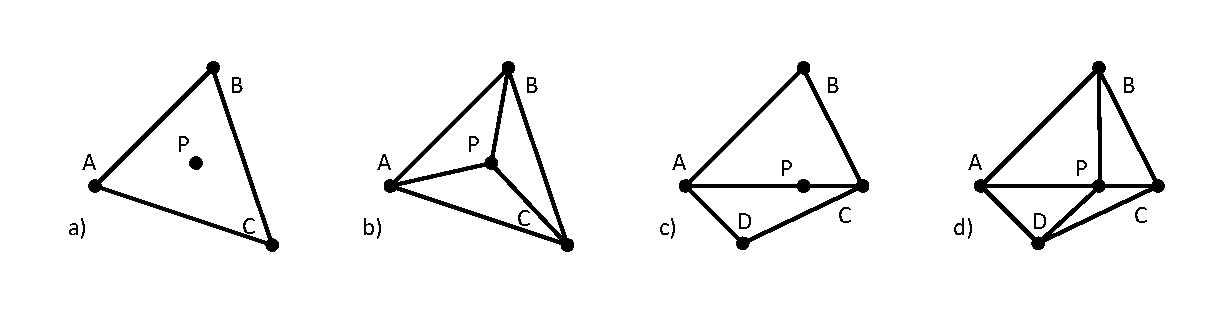
\includegraphics[width=1.0\textwidth]{pics/pic_split_s.pdf}
\captionstyle{center}\caption{Разбиение треугольников по точкам пересечения.}\label{fig:pic_split_s}
\end{figure}

\section{Удаление лишних ячеек}

\begin{figure}[h]
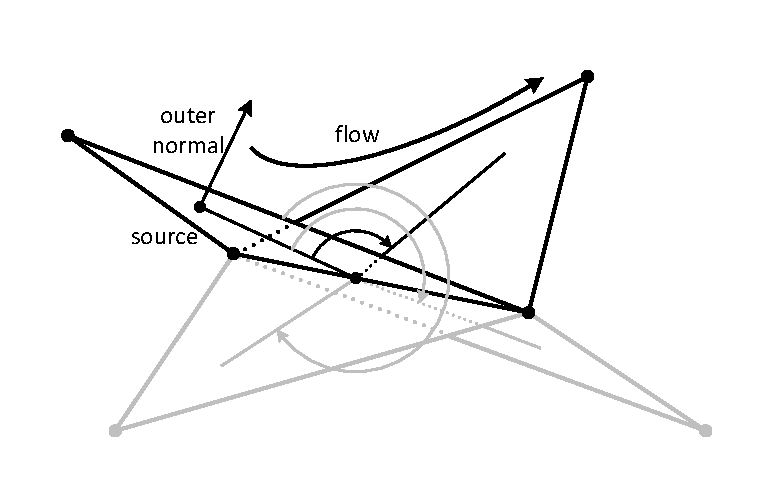
\includegraphics[width=0.7\textwidth]{pics/pic_del_extra_s.pdf}
\captionstyle{center}\caption{Удаление лишних ячеек.}\label{fig:pic_del_extra_s}
\end{figure}

При перестроении конечно-элементной (КЭ) сетки известны случаи возникновения самопересечений элементов сетки Fig.~\ref{fig:1}, что приводит сетку в негодность. Использование дефектной КЭ сетки – сетки с самопересечения не допустимо для проведения дальнейших расчетов. Отсюда возникает необходимость детектирования, локализации и устранения самопересекающихся участков.
Решение данной задачи можно свести к трем последовательным шагам:

\begin{itemize}
  \item нахождение точек самопересечения КЭ сетки;
  \item разбиение элементов КЭ сетки по точкам пересечения;
  \item удаление лишних треугольников, которые оказались внутри контура.
\end{itemize}

% Рис.1
\begin{figure}[h]
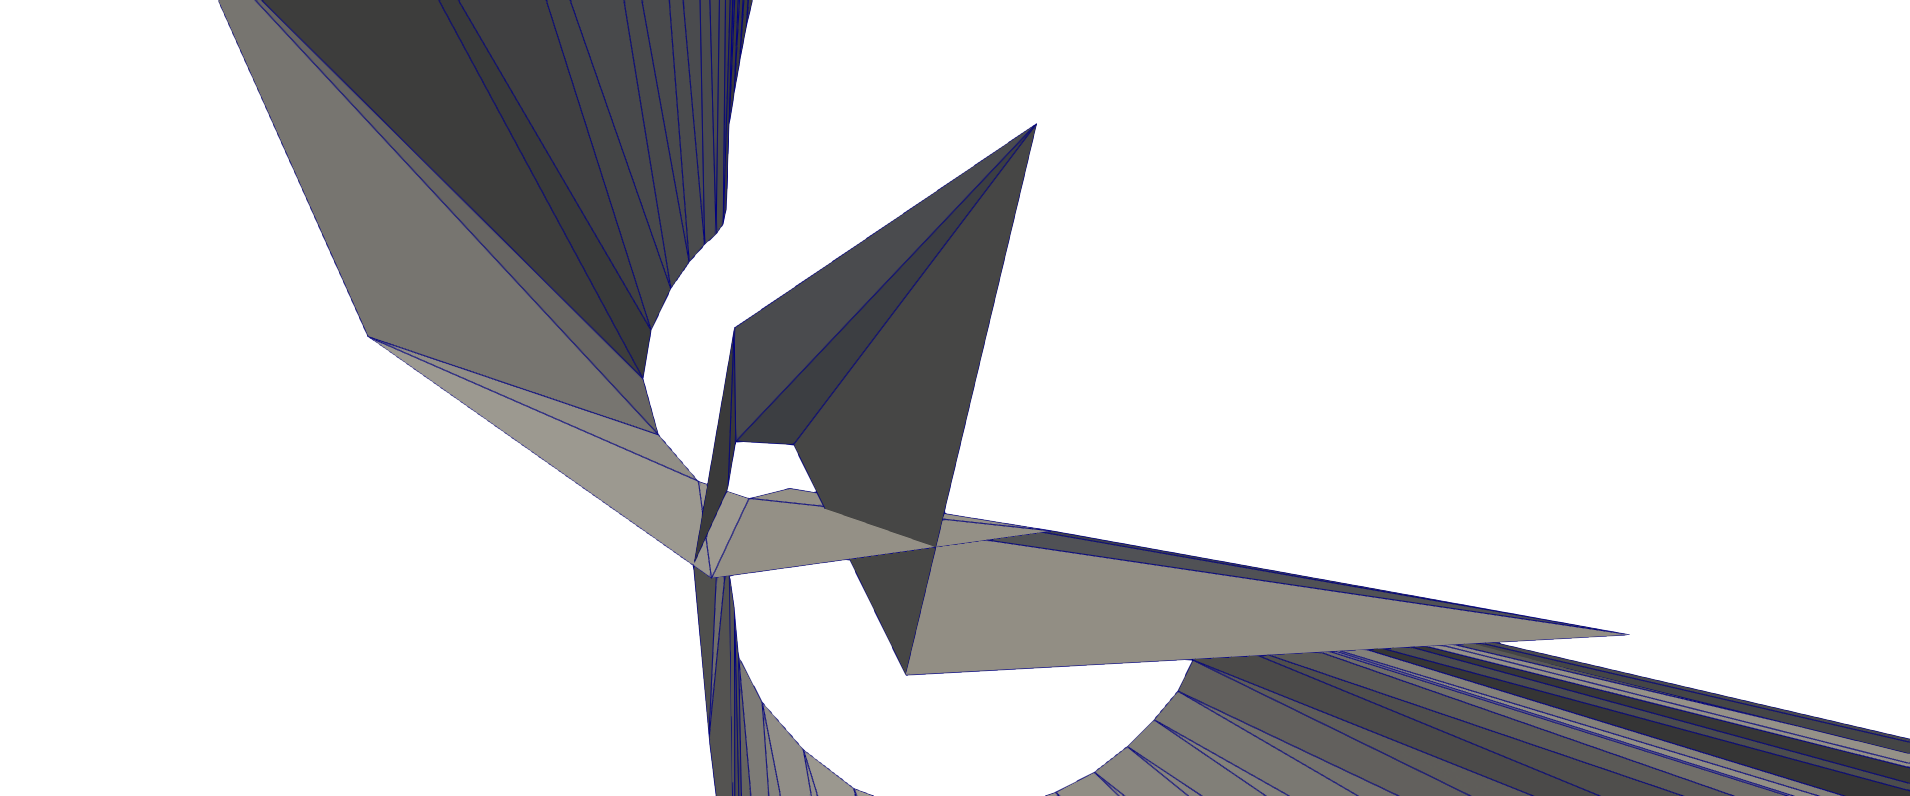
\includegraphics[width=1.0\textwidth]{pics/pic_1.png}
\captionstyle{center}\caption{КЭ сетка с подкрашенными участками самопересечений.}\label{fig:1}
\end{figure}

\section{Detection of self-intersection points of a finite element grid}

Для детектирования точки пересечения двух и более элементов сетки, необходимо сначала дать определение, что считается точками пересечения, а что нет.

Чтобы решить эту задачу, необходимо определить природу их возникновения.
В данной работе рассматривается КЭ сетка, элементами которой являются плоские треугольник. А при пересечении одного треугольника с другим как раз и возникают различные точки пересечений.
Рассмотрим случай, когда пересекающиеся треугольники находятся в различных плоскостях Fig.~\ref{fig:2}. 

% Рисунок 2. Пересечение двух треугольников в разных плоскостях.
\begin{figure}[h]
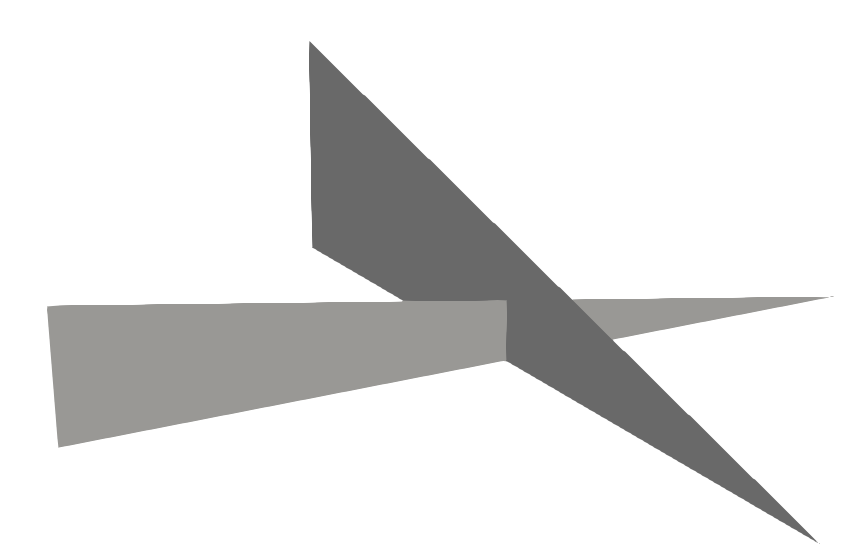
\includegraphics[width=0.6\textwidth]{pics/pic_2.png}
\captionstyle{center}\caption{Пересечение двух треугольников в разных плоскостях.}\label{fig:2}
\end{figure}

Как видно из Fig.~\ref{fig:2}, пересечение двух плоских треугольников – это пересечение двух плоскостей. Результатом пересечения двух плоскостей является линия. В частном случае, при решении задачи пересечения двух треугольников, результатом их пересечения будет прямая, ограниченная двумя точками – отрезок. Точки начала и конца данного отрезка и будут являться искомыми точками пересечения, необходимыми для перехода к следующему шагу устранения данного дефекта КЭ сетки.

Как можно понять из задачи пересечения двух плоскостей, результатом пересечения всегда является прямая, в частном случае отрезок. Но в задаче пересечения треугольников в разных плоскостях есть частный случай, когда один треугольник одной из своих вершин пересекает плоскость другого треугольника. Данный случай необходимо было упомянуть, чтобы учесть его в последующем алгоритме детектирования точек пересечений.
Второй вид пересечения треугольников – пересечение двух треугольников, находящихся в одной плоскости. Этот случай является частным в задаче пересечения двух треугольников в пространстве, но куда более сложным с точки зрения проведения анализа результатов пересечения из-за наличия куда большего количества комбинаций пересечений, которые все необходимо учитывать. 
Теперь, когда известны все возможные варианты возникновения точек пересечений двух элементов КЭ сетки, можно приступать к выбору алгоритма анализа пересечений всех треугольников в КЭ сетке.

Самый простой метод, которым можно воспользоваться и однозначно найти все пересечения треугольников – это сравнить каждый треугольник с каждым и проанализировать их взаимное расположение в пространстве на наличие точек пересечения или их отсутствие. 
Данный алгоритм имеет квадратичную сложность – $О(n^2)$, т.е. количество необходимых операций сравнения взаимного расположения двух треугольников и вычисления их точек пересечений будет зависеть от числа треугольников возведенного в квадрат. Если учесть, что в классических тепловых и аэродинамических расчетах с применение CAE систем используются КЭ сетки с количеством элементов сетки, исчисляемых тысячами или сотнями тысяч, то в итоге данный алгоритм значительно увеличит расход вычислительных ресурсов и увеличит время получения конечного результата. А это только первый шаг для решения исследуемой задачи, которая сама является одной из многих задач, которые необходимо решать при работе с КЭ сетками.
Учитывая все вышеизложенное, было принято решение использовать алгоритмы с логарифмической сложностью – $O(log_2n)$. Для реализации такого алгоритма уже не подходит сравнение каждого треугольника с каждым, потому решением стало рекурсивное сравнение между собой неких областей треугольников (далее облако), в которых потенциально есть пересекающиеся треугольники.
Для реализации рекурсивной проверки пересечений таких облаков, каждое облако образуется следующим образом. Если рассматриваемый массив элементов КЭ сетки - облако, содержит в себе больше одного элемента, то его пространство разбивается на две части (подъоблака) по длинной стороне ребра пространственного прямоугольника, описывающего все треугольники исходного массива (далее бокс) Fig.~\ref{fig:3}. Если в облаке всего один элемент КЭ сетки, то подъоблака не образуются.

% Рисунок 3. Бокс описывает пространство треугольников.
\begin{figure}[h]
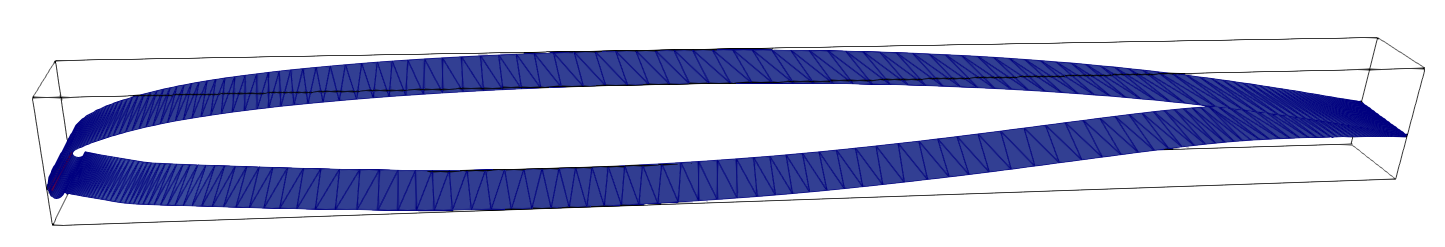
\includegraphics[width=1.0\textwidth]{pics/pic_3.png}
\captionstyle{center}\caption{Бокс, описывает пространство треугольников.}\label{fig:3}
\end{figure}

То есть исходный массив треугольников КЭ сетки теперь можно представить в виде дерева Fig.~\ref{fig:4}. Где исходный массив разбивается на два подъоблака, образуя тем самым первые две ветви дерева. Каждое их этих облаков треугольников в свою очередь содержат еще под два подъоблака – половины набора треугольников от вышестоящего облака. И такое бинарное рекурсивное образование ветвей дерева от исходного массива продолжается до тех пор, пока в облаке треугольников не останется всего один объект – один треугольник от исходной КЭ сетки, что и будет являться листьями этого дерева. 

% Рисунок 4. Древовидная структура данных КЭ сетки.
\begin{figure}[h]
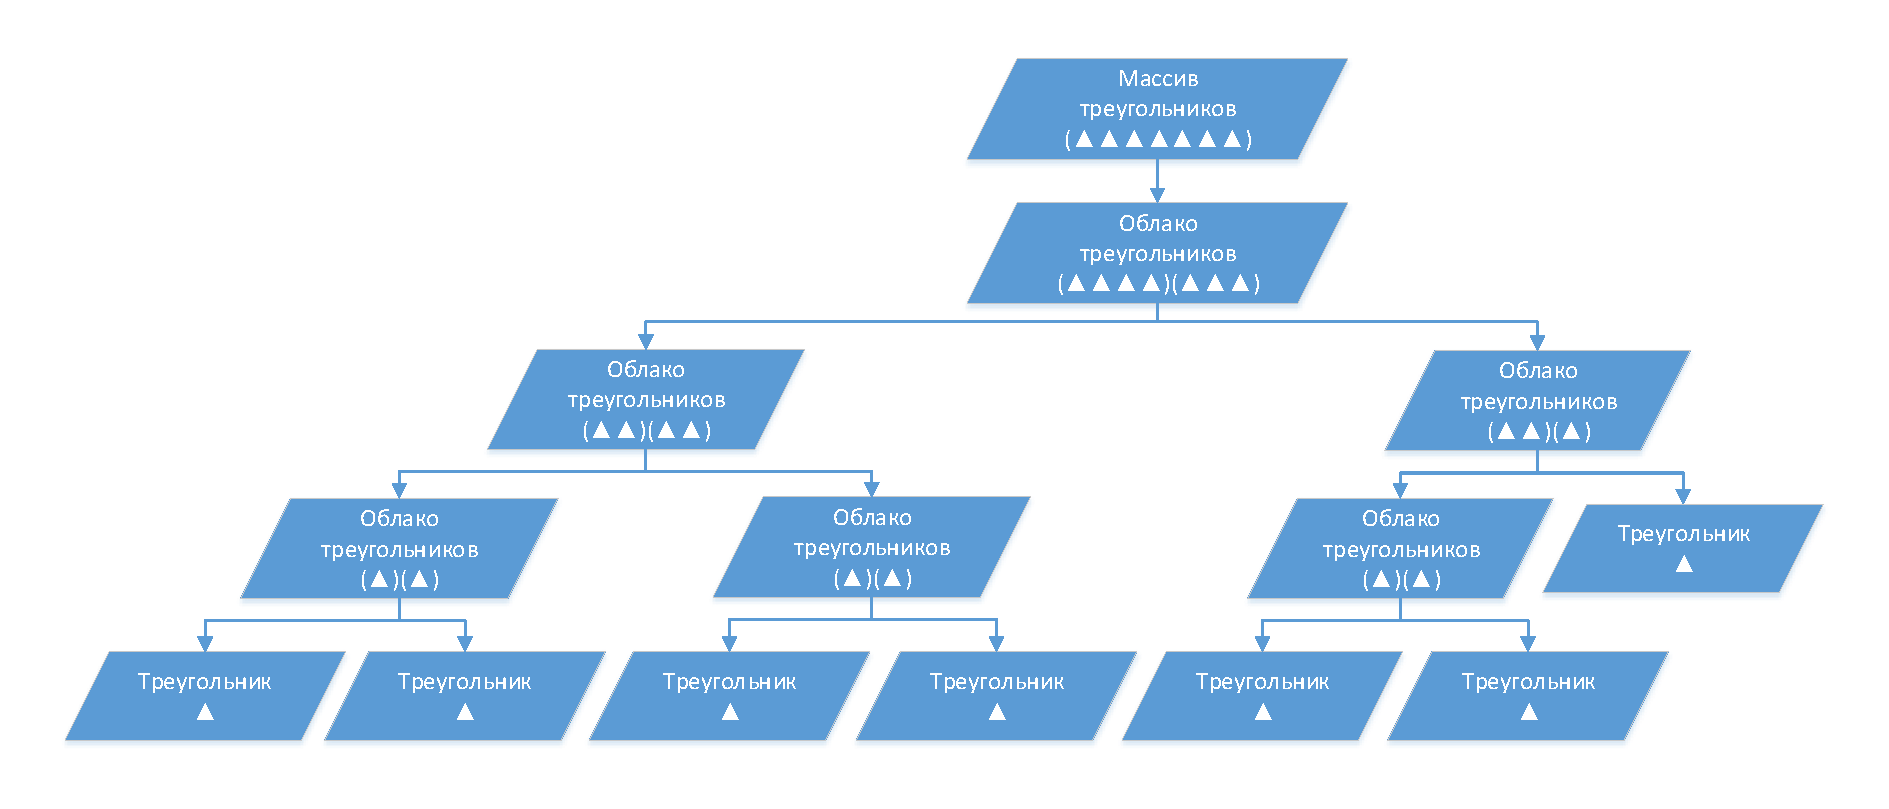
\includegraphics[width=1.0\textwidth]{pics/pic_4.pdf}
\captionstyle{center}\caption{Древовидная структура данных КЭ сетки.}\label{fig:4}
\end{figure}

Итоговый алгоритм поиска самопересечений КЭ сетки теперь можно описать следующим образом. Исходный массив элементов КЭ сетки представляется в виде дерева и далее происходит сравнение этого дерева с самим собой на предмет наличия двух пересекающихся треугольников. Данный процесс сравнения двух одинаковых деревьев происходит рекурсивно, каждый раз проверяя 4 условия.

Первое условие. Если два облака не пересекаются – их боксы не имеют общего пространства, то в этих облаках нет потенциально возможных пересечений элементов КЭ сетки.

Второе условие. Если облака пересекаются и у облака от первого дерева есть подъоблака, то с каждым подъоблаком сравнивается с облаком от второго дерева.

Третье условие. Если облака пересекаются и у облака от второго дерева есть подъоблака, то облако от первого дерева сравнивается с каждым подъоблаком.

Четвертое условие. Если облака пересекаются и у обоих облаков нет подъоблаков, то это искомые два элемента, которые потенциально пересекаются и необходимо провести анализ их взаиморасположения и выдать результат.

Такой подход позволяет быстро отбросить большие области треугольников, которые не содержат в себе потенциально пересекающихся элементов КЭ сетки.

Непосредственный анализ взаиморасположения двух треугольников – поиск их точек пересечения сводится к последовательному поиску пересечений одного треугольника с каждым ребром второго и наоборот Fig.~\ref{fig:5}, образую шесть последовательных анализов пересечений треугольника с отрезком. Далее все шесть результатов округляются до заданной точности вычислений, сортируются, отбрасываются повторяющиеся значения, формируя конечный результат – список точек пересечений двух треугольников.

Алгоритм анализа пересечений треугольника с отрезком состоит из двух основных частей: отрезок параллелен плоскости треугольника и под углом к плоскости треугольника.

% Рисунок 5. Пересечение треугольника отрезком.
\begin{figure}[h]
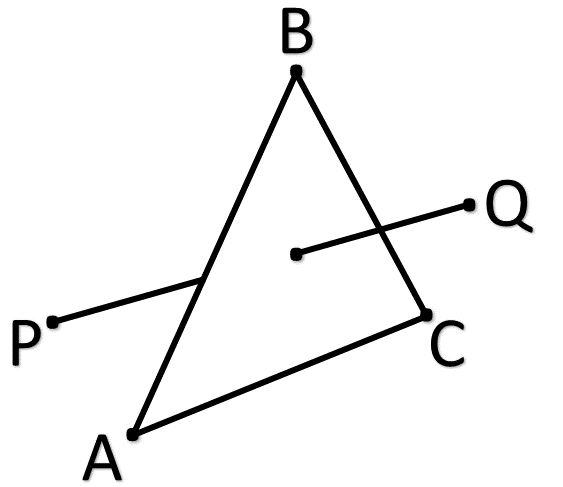
\includegraphics[width=0.3\textwidth]{pics/pic_5.png}
\captionstyle{center}\caption{Пересечение треугольника отрезком.}\label{fig:5}
\end{figure}

В случае, когда отрезок находится под углом к плоскости треугольника, задача сводится к решению системе линейных уравнений:

\[
  \begin{cases}
    A_x + (B_x - A_x)*\alpha+(C_x-A_x)*\beta=P_x+(Q_x-P_x)*\phi      \\
    A_y + (B_y - A_y)*\alpha+(C_y-A_y)*\beta=P_y+(Q_y-P_y)*\phi      \\
    A_z + (B_z - A_z)*\alpha+(C_z-A_z)*\beta=P_z+(Q_z-P_z)*\phi
  \end{cases},\eqno(1)
\]

где левая часть уравнения описывает точку, находящуюся в треугольнике $ABC$, а правая часть – точку, находящуюся на прямой $QP$. Следовательно, если левая и правая стороны системы (1) равны, то численное значение любой из сторон - это координаты точки пересечения. При этом коэффициенты треугольника - $\alpha$, $\beta$ и коэффициент отрезка – $\phi$ должны удовлетворять систему неравенств:

\[
  \begin{cases}
    \alpha \geq 0      \\
    \beta \geq 0      \\
    \alpha+\beta \leq 1\\
    0 \leq \phi \leq 
  \end{cases}.\eqno(2)
\]

В случае, когда отрезок параллелен плоскости треугольника, сначала проверяется принадлежность точек отрезка $PQ$ к плоскости, образованной треугольником АВС, путем нахождения определителя матрицы, которая описывает уравнение данной плоскости:

\[D = 
     \begin{bmatrix}
       P_x - A_x & P_y - A_y & P_z - A_z          \\
       B_x - A_x & B_y - A_y & B_z - A_z          \\
       C_x - A_x & C_y - A_y & C_z - A_z 
     \end{bmatrix},\eqno(3)
\]

где если $D$ – определитель матрицы будет равен нулю, это будет значить, что точка P принадлежит треугольнику $АВС$, а поскольку отрезок $PQ$ параллелен плоскости треугольника, то при этом условии весь отрезок принадлежит плоскости треугольника.

Далее сложность задачи снова понижается и сводится к поиску пересечений двух отрезков – анализ пересечений каждого отрезка, образующего одно из ребер треугольника $АВС$, и отрезка $PQ$. Точка пересечения в данном случае находится путем решения системы линейных уравнений:

\[
  \begin{cases}
    A_x + (B_x - A_x)*u=P_x+(Q_x-P_x)*v      \\
    A_y + (B_y - A_y)*u=P_y+(Q_y-P_y)*v      \\
    A_z + (B_z - A_z)*u=P_z+(Q_z-P_z)*v
  \end{cases},\eqno(4)
\]

где $A$, $B$ – вершины одного ребра из трех анализируемых ребер треугольника и коэффициенты каждого отрезка $u$ и $v$, значение которых должны удовлетворять систему неравенств:

\[
  \begin{cases}
    0 \leq u \leq 1\\
    0 \leq v \leq 1
  \end{cases}.\eqno(5)
\]

Но данный процесс нахождения точек пересечений отрезка с треугольником, лежащих в одной плоскости, можно немного упростить, если в начала проверить, не лежит ли одна или обе точки отрезка внутри треугольника. Это может позволить или сразу найти ответ, если отрезок лежит внутри треугольника (и избежать пустого решения, при поиске точек пересечения путем поиска пересечения каждого ребра треугольника с отрезком), или найти часть ответа, если только одна точка отрезка находится внутри треугольника.
После нахождения всех точек пересечений для каждого треугольника, получается массив треугольников и соответствующих им точек пересечения. Этих данных достаточно, чтобы приступить к следующему шагу – перестроению треугольников по точкам пересечений.
Но проведя анализ этого результирующего массива, было выявлено, что один треугольник может пересекать от одного и более треугольников за раз, что привело к тому, что в результирующем массиве треугольников и их точек пересечений есть повторяющиеся треугольники с разными точками пересечения. Для этого просто объединим все элементы массива по одинаковым треуголькам и конкатенируем их точки пересечений.

В таком упорядоченном и отфильтрованном виде элементы результирующего массива содержат в себе полноценный набор данных для перестроения всех треугольников, которые имеют пересечения.

\section{Splitting the elements of a finite element grid grid by intersection points}

Имея массив треугольников и их точек пересечения, можно простым линейным алгоритмом со сложностью O(n) рассмотреть каждый случай и перестроить все треугольники.

На верхнем уровне, алгоритм перестроения представляет собой цикл из двух фильтров, позволяющих избежать не нужных операций Fig.~\ref{fig:6}.

% Рисунок 6. Блок-схема алгоритма перестроения разбиения элементов КЭ сетки по точкам.
\begin{figure}[h]
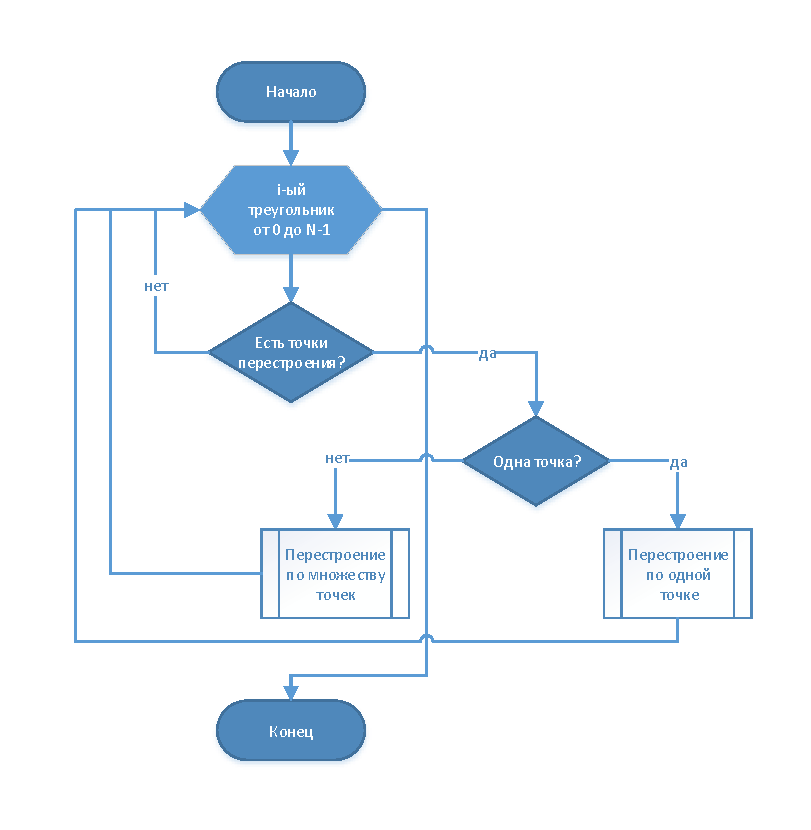
\includegraphics[width=0.8\textwidth]{pics/pic_6.pdf}
\captionstyle{center}\caption{Блок-схема алгоритма перестроения разбиения элементов КЭ сетки по точкам.}\label{fig:6}
\end{figure}

Первый фильтр проверяет принадлежность точек для перестроения к конкретным областям исследуемого треугольника: если есть точки вне треугольника или в его вершинах, то они отбрасываются.
Второй фильтр просто оценивает остались ли точки для перестроения треугольника, и если да, то данный треугольник будет перестроен.

Сам процесс перестроения в общем виде можно разбить на две части: если точек для перестроения одна, если точек для перестроения больше одной.

Если точек для перестроения больше одной, то перестроение происходит по первой точке в массиве. Результирующие треугольники, полученные после такого перестроения, и оставшиеся точки добавляются в конец списка исследуемых треугольников.

Итого этот метод перестроения треугольников и второй – перестроения по одной точке сводятся к перестроению треугольника по одной точке. Видов таких перестроений всего два – перестроение треугольника, когда тоска находится в середине треугольника (внутренней области), и перестроение треугольника, когда точка принадлежит одному из ребер треугольника.

Перестроение треугольника по точке Р, находящейся во внутренней области треугольника. На основе точки, принадлежащей внутренней области треугольника и лежащей в плоскости треугольника, формируются три новых треугольника. Для этих треугольников формируются связи с остальными элементами КЭ сетки. Старый треугольник удаляется из сетки Fig.~\ref{fig:7}.

\begin{figure}[h]
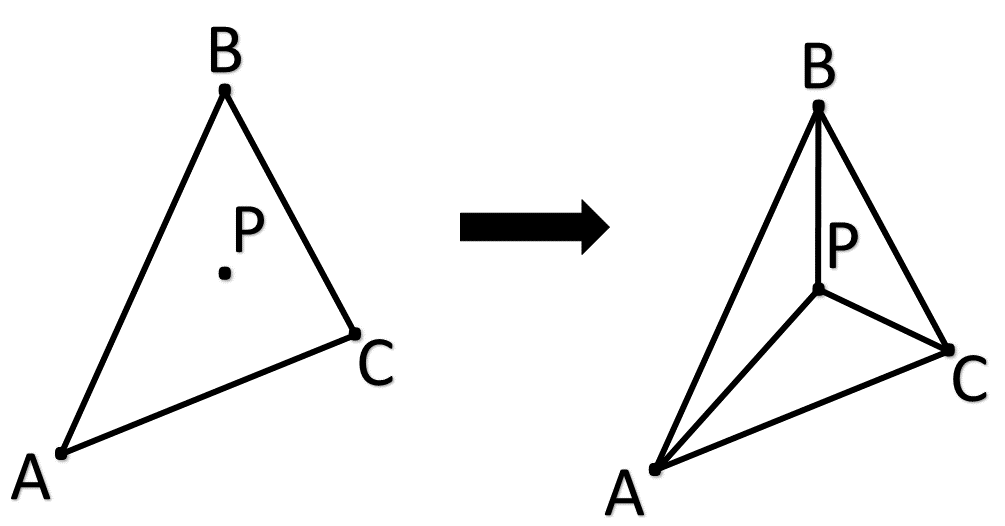
\includegraphics[width=0.5\textwidth]{pics/pic_7.png}
\captionstyle{center}\caption{Перестроение треугольника по внутренней точке пересечения.}\label{fig:7}
\end{figure}

Перестроение треугольника по точке Р, лежащей на ребре. На основе точки на ребре, происходит разбиение ребра, которому она принадлежала. А также от этой точки формируется новое ребро, соединяющее ее и противоположную ей вершину исходного треугольника. Тем самым формируются два новых треугольника на месте старого Fig.~\ref{fig:8}. Формируются связи в сетке для новых треугольников и их элементов. Исходный треугольник удаляется из сетки. Противоположный треугольник (если он есть), который прилегал к разбитому на две части ребру АС, также будет разбит на две части по этой же точке, когда до него дойдет очередь.

\begin{figure}[h]
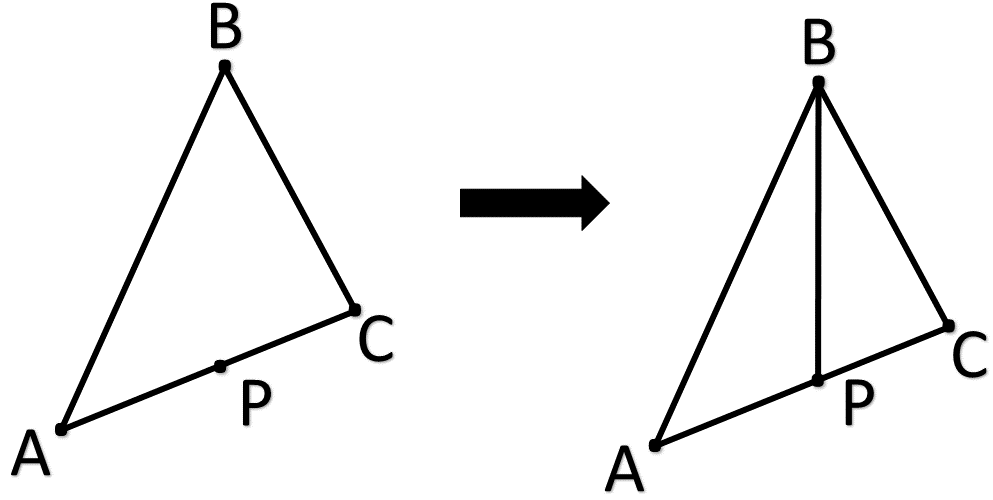
\includegraphics[width=0.5\textwidth]{pics/pic_8.png}
\captionstyle{center}\caption{Перестроение треугольника по точке на ребре.}\label{fig:8}
\end{figure}

\begin{figure}[h]
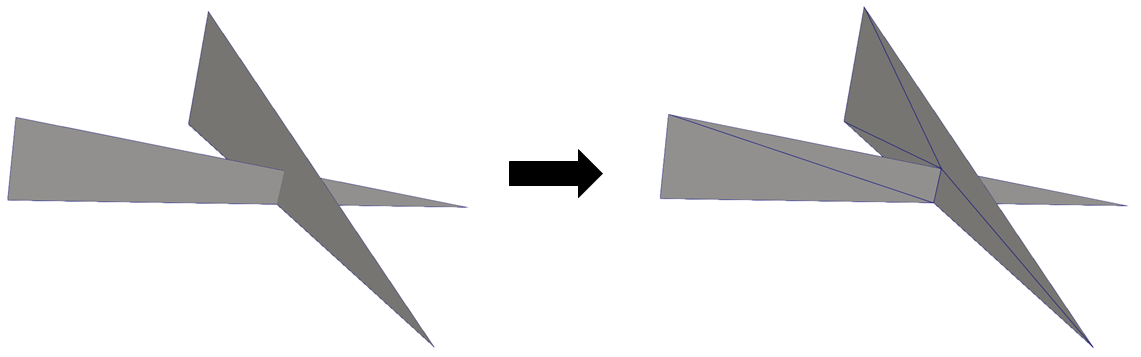
\includegraphics[width=0.8\textwidth]{pics/pic_9.png}
\captionstyle{center}\caption{Визуализация перестроения двух пересекающихся треугольников.}\label{fig:9}
\end{figure}

Результатом такого перестроения всех элементов КЭ сетки является сетка без пересечений: все треугольники, которые имели пересечения, перестроены. Теперь ранее пересеченные треугольники представляют собой наборы новых треугольников, ребра которых теперь принадлежат не двум треугольников, а четырем, а возможно и больше Fig.~\ref{fig:9}.

\section{Removing Triangles}

После устранения самопересечений описанным выше способом осталась существенная проблема - результирующая сетка в общем случае перестает быть поверхностной, а значит она непригодна для проведения расчетов, например, течения пленки воды по поверхности.

После дробления сетки в ней появились ребра, к которым примыкают более двух ячеек. Это значит, что у некоторой ячейки не может однозначным образом быть определен сосед по ребру. На Fig.~\ref{fig:10} приведена расчетная сетка после выполнения дробления ячеек и с подкрашенными проблемными ячейками (для которых не может быть однозначно определен сосед по ребру).

\begin{figure}[h]
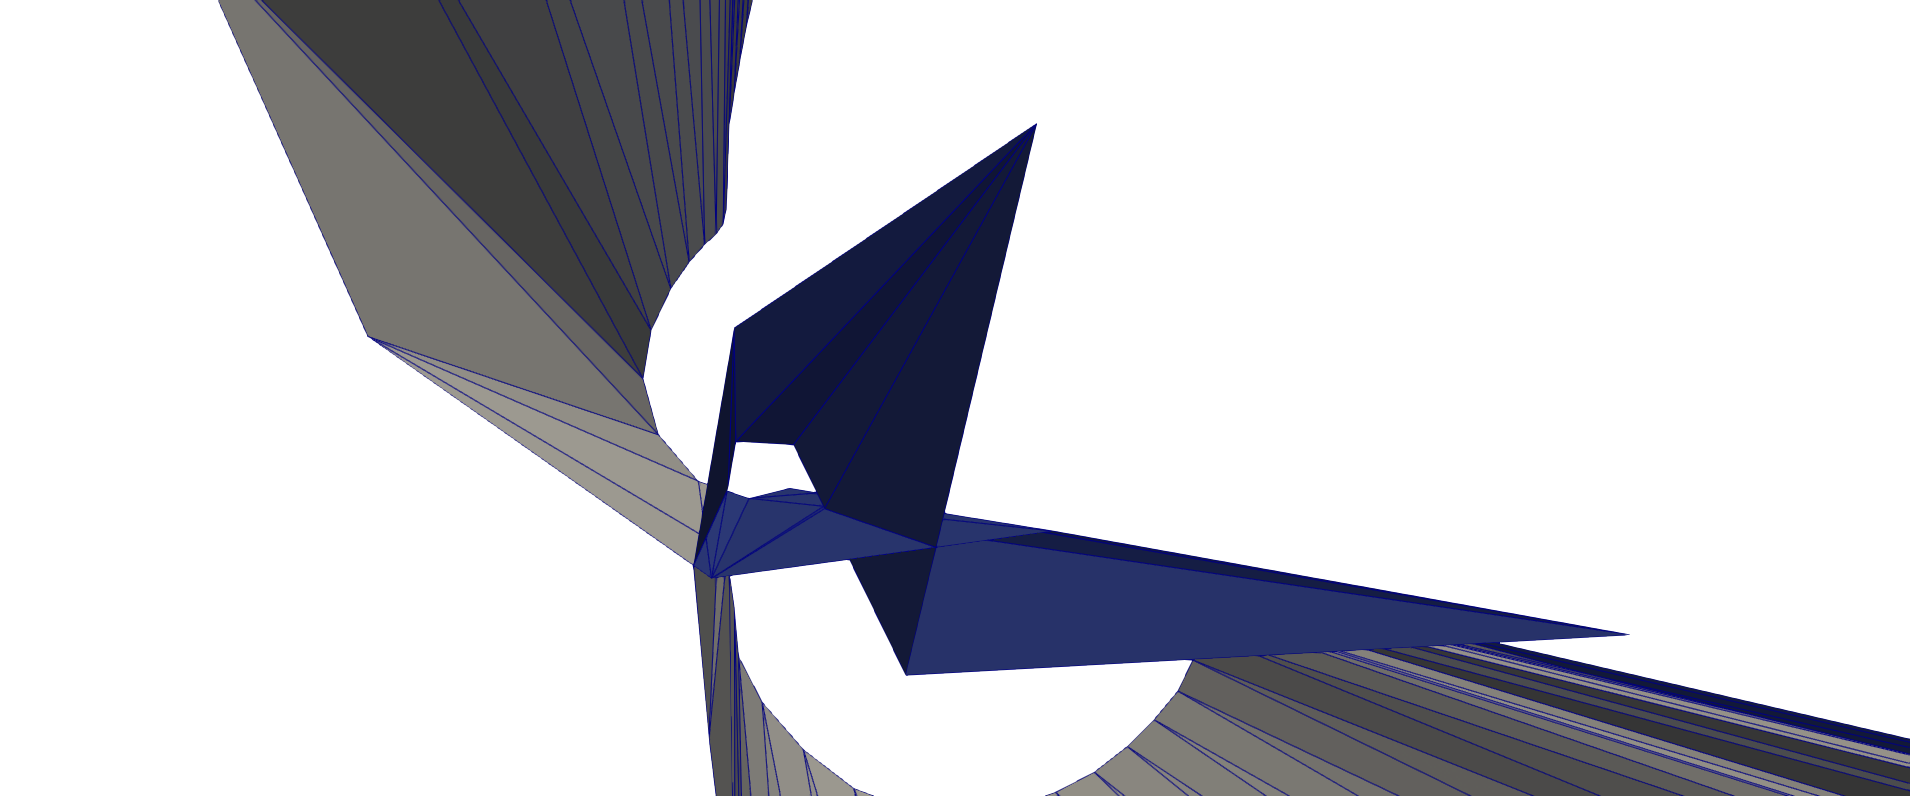
\includegraphics[width=1.0\textwidth]{pics/pic_10.png}
\captionstyle{center}\caption{Перестроенные элементы сетки с подкрашенными участками, которые необходимо удалить.}\label{fig:10}
\end{figure}

Для устранения неоднозначности некоторые из проблемных ячеек должны быть удалены из КЭ сетки, а также должны быть удалены области КЭ сетки, которые перестали быть активными (то есть такие области, до которых отсутствует доступ их заведомо валидных ячеек). Заведомо корректные ячейки сетки могут быть определены. Для построения новой поверхности необходимо выполнить обход всего графа расчетной сетки, начиная с заведомо корректных ячеек. При прохождении через ребра, в которых сходится более двух ячеек для текущей ячейки может быть выбран только один сосед. Так как в задаче расчета обледенения поверхность обтекаемого тела явно разделяет пространство на две области (тело и окружающее пространство), то в качестве соседа текущей ячейки берется та ячейка, для которой угол поворота текущей ячейки для совмещения плоскости текущей ячейки с плоскостью потенциального соседа является минимальным (при этом поворот осуществляется через половину пространства, которая соответствует окружающей среде). После выполнения обхода всей расчетной сетки по описанному алгоритму оставшиеся ячейки считаются неактивными Fig.~\ref{fig:10} и могут быть удалены.

В результате выполнения всех трех основных шагов по коррекции КЭ сетки, получаем поверхностную сетку, где для каждого элемента сетки можно однозначно определить ближайших соседей – каждое ребро элемента сетки имеет только две соседние ячейки Fig.~\ref{fig:11}.

\begin{figure}[h]
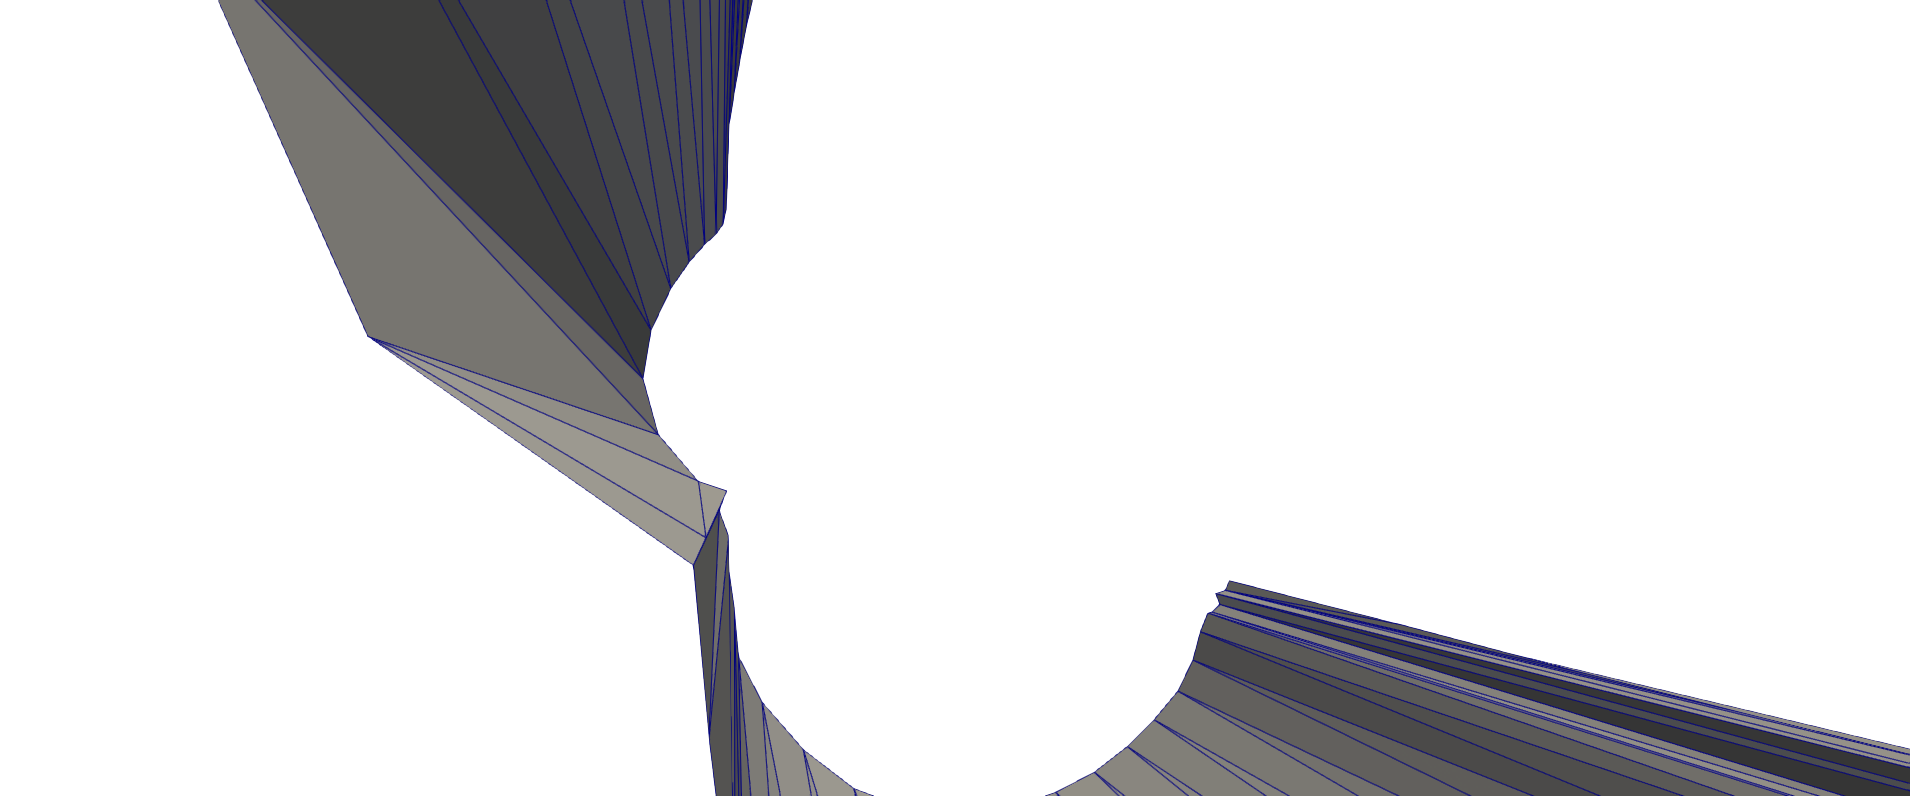
\includegraphics[width=1.0\textwidth]{pics/pic_11.png}
\captionstyle{center}\caption{Результирующая корректная КЭ сетка.}\label{fig:11}
\end{figure}

\section{Conclusion}

Предложенный алгоритм коррекции поверхностной расчетной сетки позволяет справляться с ситуациями, в которых во время конструирования ледяного нароста возникают самопересечения поверхности льда. Данная ситуация соответствует затягиванию тонких впадин на поверхности льда и не должна приводить к остановке расчета. Устранение самопересечений и удаление неактивных участков поверхностной сетки позволяет реализовать этот физически оправданный функционал и обеспечить устойчивую работу приложения по расчету ледяного нароста.

\begin{acknowledgments}
The work has been done at the JSCC RAS as part of the state assignment for the to 0580-2021-0016.
The supercomputer MVS-10P OP (Broadwell, KNL, Skylake and Cascade Lake segments), located at the JSCC RAS, was used during the research.
\end{acknowledgments}

\begin{thebibliography}{99}

% ice accretion task

\bibitem{Myers}
\refitem{article}
T.~Myers, \textquotedblleft Extension to the Messinger model for aircraft icing,\textquotedblright \ AIAA J. \textbf{39}, 211--218 (2001).

\bibitem{Farzaneh}
\refitem{article}
P.~Farzaneh and G.~Bouchard, \textquotedblleft Modeling a water flow on an icing surface,\textquotedblright \ in \textit{Proceedings of the International Workshop on Atmospheric Icing of Structures IWAIS XI, Montr\'eal, 2005}.

\bibitem{Dong}
\refitem{article}
W.~Dong, J.~Zhu, and X.~Min, \textquotedblleft Calculation of the heat transfer and temperature on the aircraft anti-icing surface,\textquotedblleft \ in \textit{Proceedings of the 27th International Congress of the Aeronautical Sciences, 2010}.

\bibitem{Beaugendre}
\refitem{misc}
H.~Beaugendre, \textquotedblleft A PDE-based approach to in-flight ice accretion,\textquotedblright \ PhD Thesis (Dep. of Mech. Eng., McGill Univ., Montr\'eal, Qu\'ebec, 2003).

% ice accretion software

\bibitem{Bourgault}
\refitem{article}
Y.~Bourgault, H.~Beaugendre, and W.~Habashi, \textquotedblleft Development of a shallow-water icing model in FENSAP-ICE,\textquotedblright \ J. Aircraft \textbf{37}, 640--646 (2000).

\bibitem{Wright}
\refitem{article}
W.~Wright, P.~Struck, T.~Bartkus, and G.~Addy, \textquotedblleft Recent advances in the LEWICE icing model,\textquotedblright \ SAE Int. Technical Paper (2015).

\bibitem{Beld}
\refitem{misc}
E.~Beld, \textquotedblleft Droplet impingement and film layer modeling as a basis for aircraft icing simulations in OpenFOAM,\textquotedblright \ Internship Report (Eng. Fluid Dynamics Department, Univ. Twente, 2013).

\bibitem{Domingos}
\refitem{article}
R.~Domingos and S.~Silva, \textquotedblleft 3D computational methodology for bleed air ice protection system parametric analysis,\textquotedblright \ SAE Int. technical paper (2015).

\bibitem{Aksenov}
\refitem{article}
A.~A.~Aksenov, P.~M.~Byvaltsev, S.~V.~Zhluktov, K.~E.~Sorokin, A.~A.~Babulin, and V.~I.~Shevyakov, \textquotedblleft Numerical simulation of ice accretion on airplane surface,\textquotedblright \ in \textit{Proceedings of AIP Conference, 2019}.

% remeshing

\bibitem{BourgaultCote}
\refitem{article}
S.~Bourgault-C\^ot\'e, K.~Hasanzadeh, P.~Lavoie, and E.~Laurendeau, \textquotedblleft Multi-layer icing methodologies for conservative ice growth,\textquotedblright \ in \textit{Proceedings of 7th European Conference for Aeronautics and Aerospace Sciences EUCASS, 2017}.

\bibitem{Fortin}
\refitem{article}
G.~Fortin, A.~Ilinca, J.-L.~Laforte, and V.~Brandi, \textquotedblleft New roughness computation method and geometric accretion model for airfoil icing,\textquotedblright \ J. Aircraft \textbf{41}, 119--1127 (2004).

\bibitem{Thompson}
\refitem{article}
D.~Thompson, X.~Tong, Q.~Arnoldus, E.~Collins, D.~McLaurin, and E.~Luke, \textquotedblleft Discrete surface evolution and mesh deformation for aircraft icing applications,\textquotedblright \ in \textit{Proceedings of 5th AIAA Atmospheric and Space Environments Conference, 2013}.

\bibitem{Tong}
\refitem{article}
X.~Tong, D.~Thompson, Q.~Arnoldus, E.~Collins, and E.~Luke, \textquotedblleft Three-dimensional surface evolution and mesh deformation for aircraft icing applications,\textquotedblright \ J. Aircraft \textbf{54}, 1--17 (2016).

% self-intersections elimination

\bibitem{Charton}
\refitem{article}
J.~Charton, S.~Baek, and Y.~Kim, \textquotedblleft Mesh repairing using topology graphs,\textquotedblright \ J. of Computational Design and Engineering \textbf{8}, 251--267 (2021).

\bibitem{Jung}
\refitem{article}
W.~Jung, H.~Shin, and B.~K.~Choi, \textquotedblleft Self-intersection removal in triangular mesh offsettings,\textquotedblright \ CAD J. \textbf{1}, 477--484 (2004).

\bibitem{Skorkovska}
\refitem{article}
V.~Skorkovsk\'a, I.~Kolingerov\'a, and B.~Benes, \textquotedblleft A simple and robust approach to computation of meshes intersection,\textquotedblright \ in \textit{Proceedings of the 13th International Joint Conference on Computer Vision, Imaging and Computer Graphics Theory and Applications VISIGRAPP, 2018}.

\end{thebibliography}

\end{document}
